%%
%% Automatically generated file from DocOnce source
%% (https://github.com/hplgit/doconce/)
%%
%%


%-------------------- begin preamble ----------------------

\documentclass[%
oneside,                 % oneside: electronic viewing, twoside: printing
final,                   % draft: marks overfull hboxes, figures with paths
10pt,norsk]{article}

\listfiles               % print all files needed to compile this document

\usepackage{relsize,makeidx,color,setspace,amsmath,amsfonts,amssymb}
\usepackage[table]{xcolor}
\usepackage{bm,ltablex,microtype}

\usepackage[pdftex]{graphicx}

% Movies are handled by the href package
\newenvironment{doconce:movie}{}{}
\newcounter{doconce:movie:counter}


\usepackage[T1]{fontenc}
%\usepackage[latin1]{inputenc}
\usepackage{ucs}
\usepackage[utf8x]{inputenc}

\usepackage{lmodern}         % Latin Modern fonts derived from Computer Modern

% Hyperlinks in PDF:
\definecolor{linkcolor}{rgb}{0,0,0.4}
\usepackage{hyperref}
\hypersetup{
    breaklinks=true,
    colorlinks=true,
    linkcolor=linkcolor,
    urlcolor=linkcolor,
    citecolor=black,
    filecolor=black,
    %filecolor=blue,
    pdfmenubar=true,
    pdftoolbar=true,
    bookmarksdepth=3   % Uncomment (and tweak) for PDF bookmarks with more levels than the TOC
    }
%\hyperbaseurl{}   % hyperlinks are relative to this root

\setcounter{tocdepth}{2}  % levels in table of contents

% Tricks for having figures close to where they are defined:
% 1. define less restrictive rules for where to put figures
\setcounter{topnumber}{2}
\setcounter{bottomnumber}{2}
\setcounter{totalnumber}{4}
\renewcommand{\topfraction}{0.95}
\renewcommand{\bottomfraction}{0.95}
\renewcommand{\textfraction}{0}
\renewcommand{\floatpagefraction}{0.75}
% floatpagefraction must always be less than topfraction!
% 2. ensure all figures are flushed before next section
\usepackage[section]{placeins}
% 3. enable begin{figure}[H] (often leads to ugly pagebreaks)
%\usepackage{float}\restylefloat{figure}

% prevent orhpans and widows
\clubpenalty = 10000
\widowpenalty = 10000

% --- end of standard preamble for documents ---


\usepackage[norsk]{babel}

% insert custom LaTeX commands...

\raggedbottom
\makeindex
\usepackage[totoc]{idxlayout}   % for index in the toc
\usepackage[nottoc]{tocbibind}  % for references/bibliography in the toc

%-------------------- end preamble ----------------------

\begin{document}

% matching end for #ifdef PREAMBLE


% ------------------- main content ----------------------



% ----------------- title -------------------------

\thispagestyle{empty}

\begin{center}
{\LARGE\bf
\begin{spacing}{1.25}
Spennende kombinasjoner av informatikk og andre realfag
\end{spacing}
}
\end{center}

% ----------------- author(s) -------------------------

\begin{center}
{\bf - hvorfor og hvordan kan programmering kombineres med de andre realfagene${}^{}$} \\ [0mm]
\end{center}

\begin{center}
% List of all institutions:
\end{center}
    
% ----------------- end author(s) -------------------------
% AUTHOR: Johan Hake IT og Fysikk-lærer på Oslo katedralskole

% --- begin date ---
\begin{center}
29. mars 2016
\end{center}
% --- end date ---

\vspace{1cm}


% !split

\section*{Hvorfor og hvordan kan programmering kombineres med de andre realfagene}

\paragraph{Oversikt.}
\begin{itemize}
\item Hvordan har jeg brukt informatikk og programmering i medisinsk hjerteforskning?

\item Hvorfor programmering?

\item Informatikk og programmering i læreplanen idag og hva sier Ludvigsen?

\item Kortkurs i matematisk modellering

\item Fremtiden?
\end{itemize}

\noindent
% !split

\section*{Hjerte ABC: Hvert hjerteslag startes og synkroniseres av et elektrisk signal}



% inline figure
\centerline{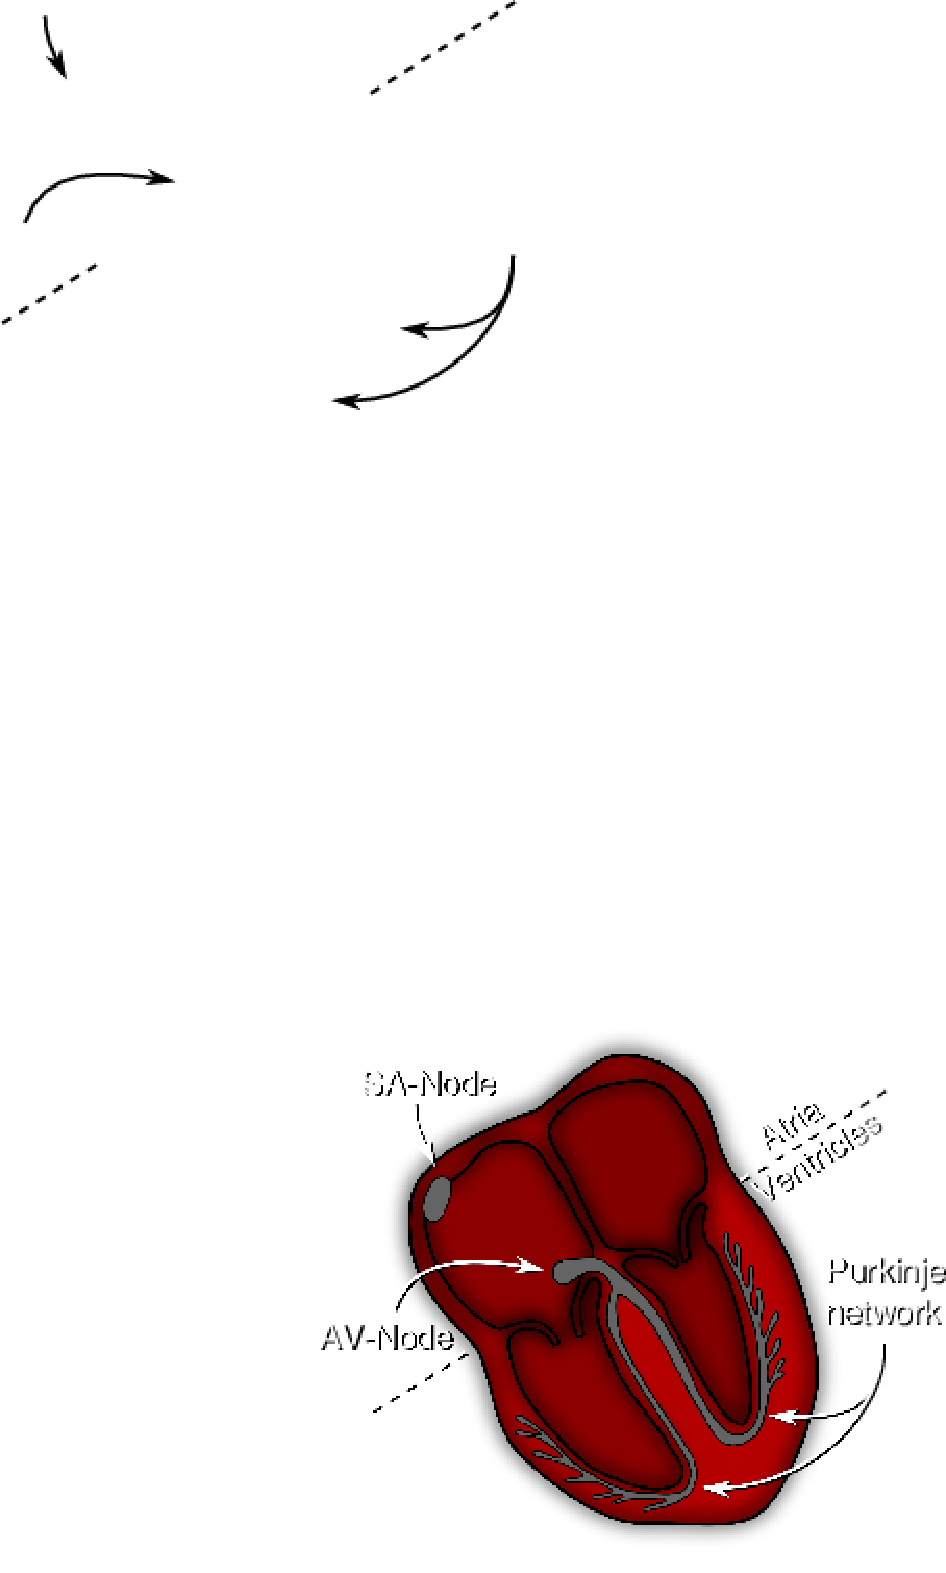
\includegraphics[width=0.9\linewidth]{fig/heart_scetch.pdf}}




% !split
\section*{Hjerte ABC: Det elektriske signalet er det vi måler gjennom EKG}



% inline figure
\centerline{
\includegraphics[width=0.9\linewidth]{fig/ecg.jpg}}



% !split

\section*{Hjerte ABC: I hver celle trigger det elektriske signalet en forsinket sammentrekning}

% !bslidecell 00
\begin{itemize}
\item Kalsium gir cellen signalet om at sammentrekningen skal starte
\end{itemize}

\noindent
% !eslidecell

% !bslidecell 01


% inline figure
\centerline{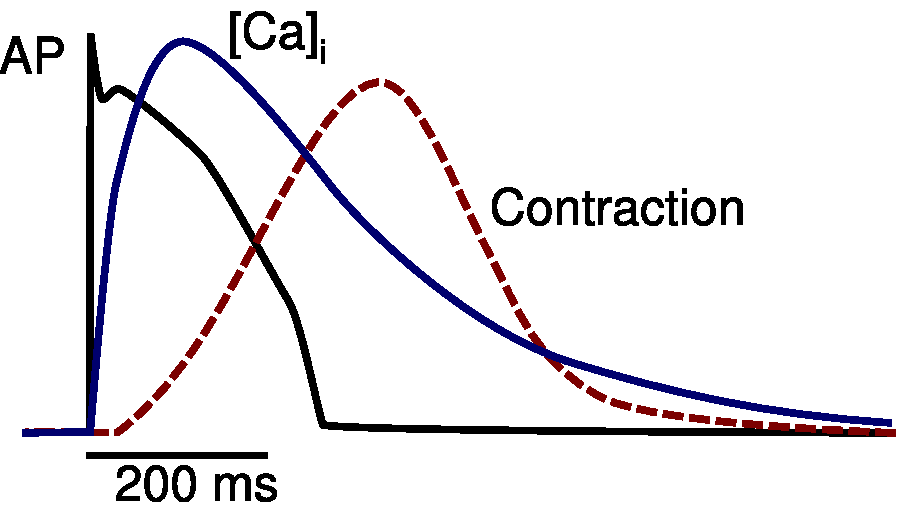
\includegraphics[width=0.9\linewidth]{fig/AP_Ca_contraction.pdf}}



% !eslidecell

% !split

\section*{Hjerte ABC: I hver celle trigger det elektriske signalet en forsinket sammentrekning}

% !bslidecell 00
\begin{itemize}
\item Kalsium gir cellen signalet om at sammentrekningen skal starte

\item Kalsium slippes inn i cellen gjennom egne ionekanaler
\end{itemize}

\noindent
% !eslidecell

% !bslidecell 01


% inline figure
\centerline{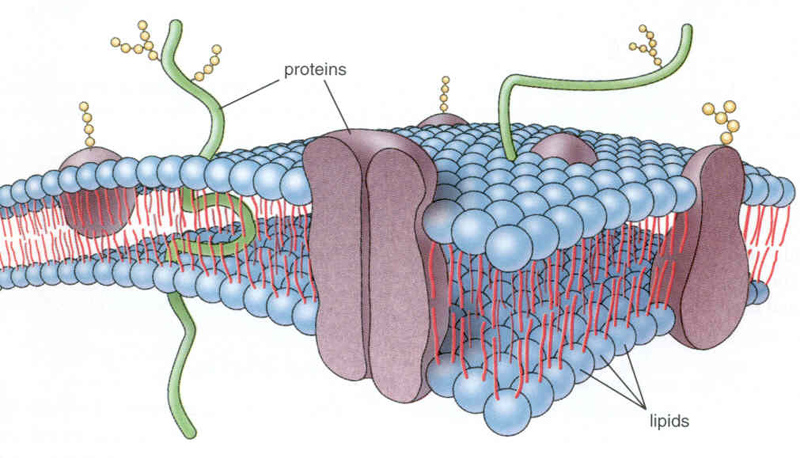
\includegraphics[width=0.9\linewidth]{fig/cell_membrane.jpg}}



% !eslidecell

% !split

\paragraph{Hvor mye kalsium som kommer ut bestemmes av en komplisert kombinasjon av geometri og kanalfunksjon.}
% inline figure
\centerline{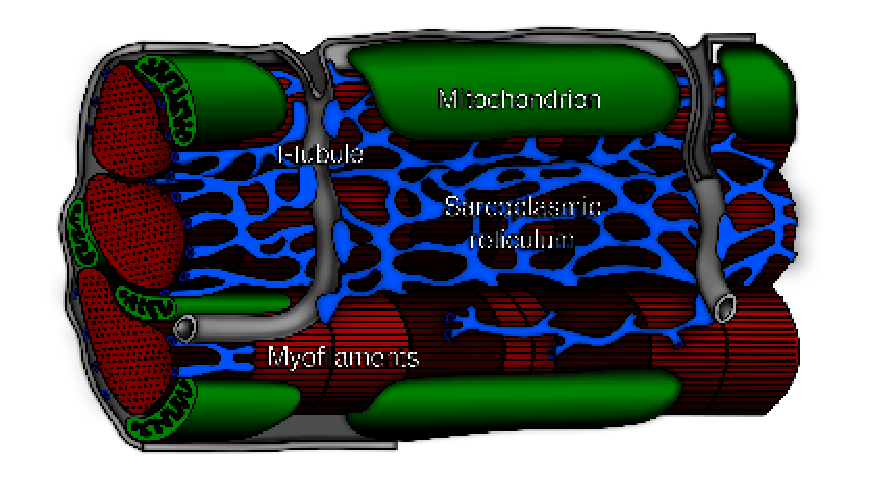
\includegraphics[width=0.9\linewidth]{fig/sarcomere_nice_black.pdf}}



\begin{itemize}
\item Vi har ikke full kvantiatativ forståelse av hva som kontrollerer
  hvor mye kalsium som kommer inn i cellen for hvert hjerteslag
\end{itemize}

\noindent
% !split
\paragraph{Selve kalsiumet kommer inn i cellen i rundt 20 000 ulike områder som er for små til å studeres i fysiologiske eksperimenter.}
% inline figure
\centerline{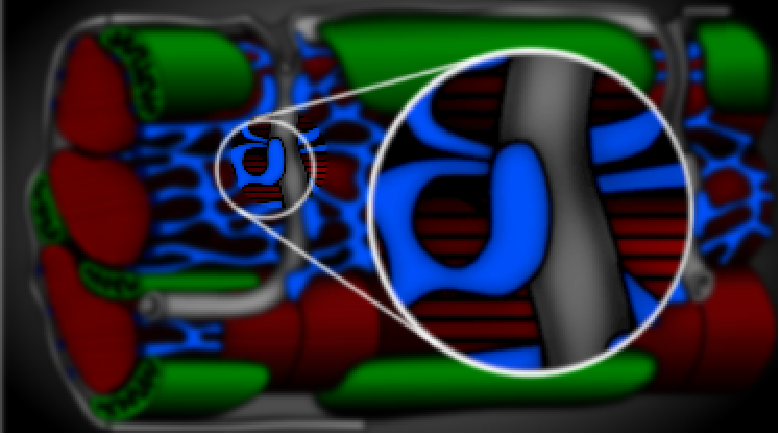
\includegraphics[width=0.9\linewidth]{fig/sarcomere_nice_black_blowup.pdf}}



\begin{itemize}
\item Gjennom matematisk modellering kan vi gi sykehusene svar på noen
  spørsmål de ikke kan få svar på gjennom egne målinger
\end{itemize}

\noindent
% !split


\paragraph{Fra et sett med bilder fra et elektronmikroskop lagde jeg en geometrisk modell av et av disse 20 000 områdene.}
\begin{doconce:movie}
\refstepcounter{doconce:movie:counter}
\begin{quote}
% link to external viewer
Movie \arabic{doconce:movie:counter}:  \href{run:fig/segmentation_2.mp4}{\nolinkurl{fig/segmentation_2.mp4}}
\end{quote}
\end{doconce:movie}


% !split


\paragraph{Den geometriske modellen ble så delt opp i flere mindre deler (diskretisert).}
\begin{doconce:movie}
\refstepcounter{doconce:movie:counter}
\begin{quote}
% link to external viewer
Movie \arabic{doconce:movie:counter}:  \href{run:fig/Tetrahedralized.mp4}{\nolinkurl{fig/Tetrahedralized.mp4}}
\end{quote}
\end{doconce:movie}


% !split

\paragraph{Til slutt beskrev jeg selve kalsiumdynamikken med en matematisk modell som ble løst for ulike parameterverdier.}
\begin{doconce:movie}
\refstepcounter{doconce:movie:counter}
\begin{quote}
% link to external viewer
Movie \arabic{doconce:movie:counter}:  \href{run:fig/fluo_spark_2.mp4}{\nolinkurl{fig/fluo_spark_2.mp4}}
\end{quote}
\end{doconce:movie}


% !split

\section*{Hva fra dette eksemplet er overførbart til bruk av IT og programmering på VGS?}

% !bpop
\begin{itemize}
\item Som motivasjon til å:
\begin{itemize}

  \item lære seg programmering

  \item jobbe med matematisk modellering

  \item arbeide tverrfaglig

\end{itemize}

\noindent
\item Sette søkelys på hvilke kunnskaper elevene trenger for å arbeide med matematisk modellering i ulike realfag
\end{itemize}

\noindent
% !epop

% !split

\paragraph{Holder det ikke med de digitale ferdighetene slik vi kjenner dem fra grunnleggende ferdigheter i læreplanen?}
% !bpop
\begin{itemize}
\item Digitale ferdigheter er en altfor generell betegnelse for å dekke behovet av spesifikk programmeringskompetanse

\item Det handler om mye mer enn å bare ta digital teknologi i bruk

\item Eleven vil forstå mer av den digitale teknologien hvis hen har utviklet den selv

\item I tilegg gir programmering eleven kunnskaper om problemløsning, jmf oppgaveløsning/forsøk i andre realfag
\end{itemize}

\noindent
% !epop


% !split

\paragraph{Programmering og IT er et lite fag i norsk skole og risikerer å fortsett være det. Men det finnes lyspunkter!}
% inline figure
\centerline{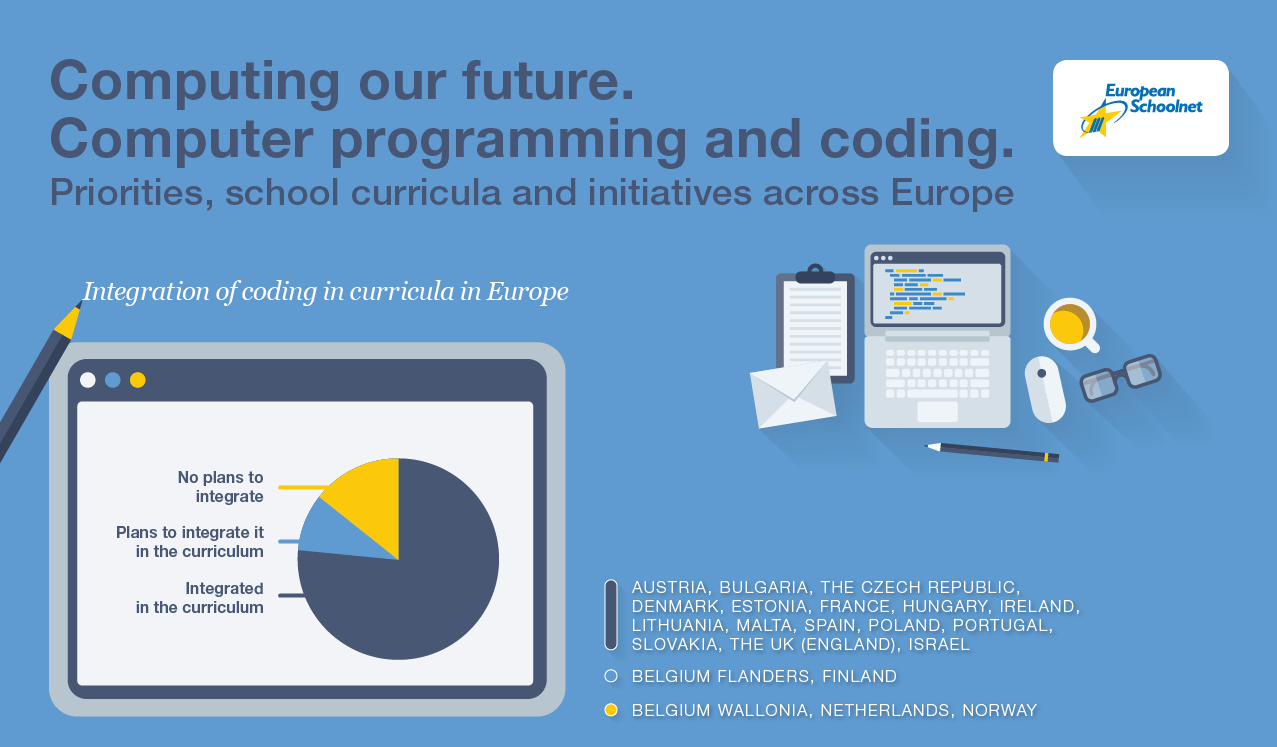
\includegraphics[width=0.9\linewidth]{fig/computing_our_future.png}}



\begin{itemize}
\item Helt nytt (1.2.16) forsøk med valgvalg i programmering i \href{{http://www.udir.no/Lareplaner/Forsok-og-pagaende-arbeid/forsok-med-programmering-som-valgfag}}{grunnskolen}

\item \href{{http://kidsakoder.no}}{Lær kidsa kode}
\end{itemize}

\noindent
% !split

\paragraph{Ludvigsen-utvalget understreker viktigheten av digital kompetanse men sier ikke noe spesifikt om IT eller programmering som eget fag (foreløpig).}
% !bslidecell 00
\begin{itemize}
\item "Matematikk, statistikk og informatikk vil bli mer og mer fremtredende innenfor klassiske naturvitenskapelige disipliner som biologi, fysikk, kjemi og geofag." (s 54)
\begin{itemize}

 \item Men det følges ikke opp med mer spesifikke tanker om informatikk. Derimot om matematikk.

\end{itemize}

\noindent
\item Ordene kode/koding programmere/programmering finnes ikke noen steder i utredningen.
\end{itemize}

\noindent
% !eslidecell
% !bslidecell 01


% inline figure
\centerline{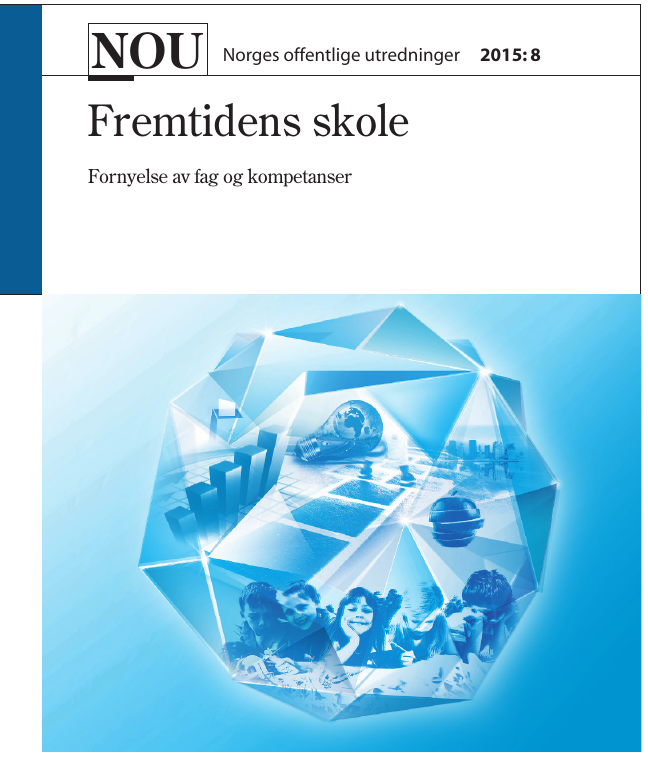
\includegraphics[width=0.9\linewidth]{fig/ludvigsen.png}}


% !eslidecell
% !split

\paragraph{Vi har et programmeringsfag i skolen idag, IT2, men det er mer rettet mot multimedia enn mot de andre realfagene og lar seg ikke lett kombineres med matematisk modellering.}
\begin{itemize}
\item Disse eksemplene er meget læreplans-relevante (EKSAMENS?!) for IT2 men de har kanskje ikke allverdens med realfag å gjøre?
\begin{itemize}

 \item \href{{kode/fugler.html}}{Fuglequiz}

 \item \href{{kode/oppgaver_animasjon_9.html}}{Rudolf}
\end{itemize}

\noindent
\end{itemize}

\noindent
% !split

\paragraph{Hvordan kan matematisk modellering og programmering integrerers i dagens realfag?}
\begin{itemize}
\item Vi bruker allerede matematisk modellering i mange fag!
\begin{itemize}

 \item Men vi tilbyr oftest bare analytiske løsninger
\end{itemize}

\noindent
\end{itemize}

\noindent
% !bpop
\begin{itemize}
\item Bevegelseslikningene for konstant aksellerasjon i fysikk: $v(t)= v_0 + a\,t;\; s = v_0\,t + a\,t^2/2$

\item S-kurven for biologiske bestand: $Y(t)= \frac{M}{1-e^{-rt}}$

\item Kjemisk likevekt: $\mathrm{K_p=\frac{[NH_3]^2}{[N_2]\cdot[H_2]^3}}$

\item Disse funksjonene og likevektsløsningen er spesialtilfeller av løsninger på differensiallikninger som kommer fra matematisk modellering

\item Hvis de skal løses analytisk må forholdene være enkle.

\item Forholdsvis enkle numeriske skjema kan brukes for å løse de opprinnelige likningene og i tillegg gjøre dem mer relevante
\end{itemize}

\noindent
% !epop

% !split

\paragraph{Løsninger man får fra numeriske skjema skiller seg fra analytiske funksjoner gjennom at vi bare kjenner løsningen på diskrete punkter i tid (og rom).}
% !bslidecell 00 0.4
\begin{itemize}
\item Hvis $\hat{t}$ er en liste (vektor) med tidspunkter
\end{itemize}

\noindent
\[\hat{t}=[0, 0.2, \ldots, 1.0]\]
\begin{itemize}
\item kan $y$ representere verdiene til en funksjon $f(\hat{t})$ i disse punktene.
\end{itemize}

\noindent
% !eslidecell

% !bslidecell 01 0.6


% inline figure
\centerline{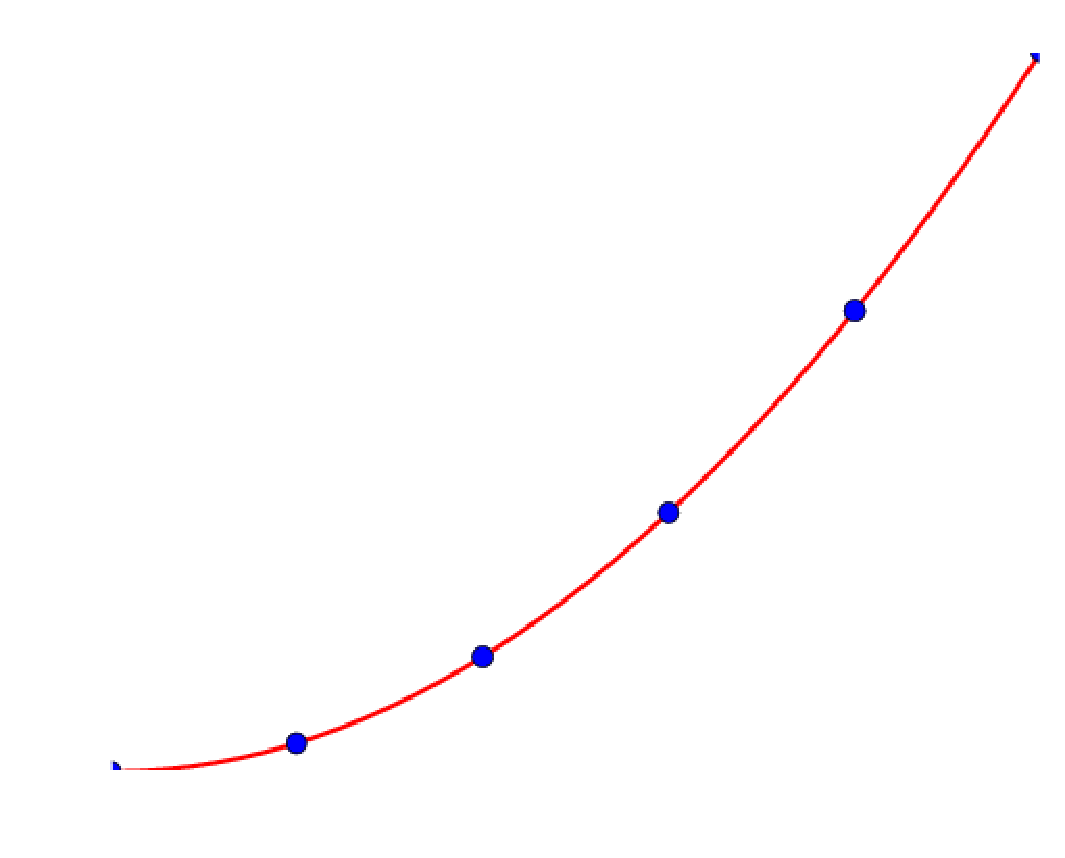
\includegraphics[width=0.6\linewidth]{fig/diskret_funksjon.pdf}}


% !eslidecell

% !split

\paragraph{Differensiallikninger finner vi i alle realfag og de kan løses med numeriske skjema som kan implementeres i et program.}
\begin{itemize}
\item Hovedidéen er at vi gjennom differensiallikningen vet hvor mye en funksjon endrer seg når tiden endrer seg litt.
\end{itemize}

\noindent
% !bpop
\begin{itemize}
\item Hvis $df(t)$ er en funksjon som gir den deriverte av $y$, $\frac{dy}{dt}$, ved tiden $t$ kan vi skrive:

\item $\frac{dy}{dt}=df(t)\simeq \frac{\Delta y}{\Delta t}=>$

\item $\Delta y = df(t) \Delta t$. Her er en liten forandring i $y$, $\Delta y$ gitt ved en liten forandring i $t$, $\Delta t$.

\item Hvis vi nå har en liste med $N+1$ tidspunkter $t=[t_0, t_1, \ldots, t_N]$ hvor hvert tidspunkt gis fra det forrige som: $t_{n+1}=t_n+\Delta t$

\item kan vi formulere den neste funksjonsverdien, $y_{n+1}$ fra det forrige, $y_{n}$ gjennom: $y_{n+1}=y_n+\Delta y_n=y_n+df(t_n) \Delta t$

\item Ofte er den deriverte avhengig av funksjonsverdien: $y_n=y_n+df(t_n, y_n)$

\item Vi har et numerisk skjema!
\end{itemize}

\noindent
% !epop

% !split

\paragraph{Visualisering av det numeriske skjemaet med $y_n$, $\Delta y_n$.}
% inline figure
\centerline{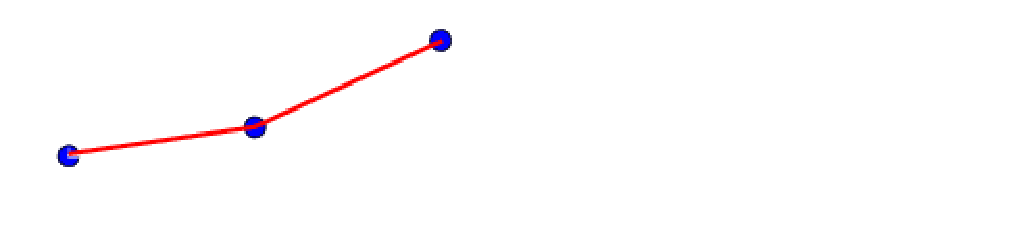
\includegraphics[width=0.9\linewidth]{fig/diskret_funksjon_0.pdf}}



\begin{itemize}
\item Gitt at vi har regnet ut 3 punkter: $y_0$, $y_1$, og $y_2$
\end{itemize}

\noindent
% !split
\paragraph{Visualisering av det numeriske skjemaet med $y_n$, $\Delta y_n$.}
% inline figure
\centerline{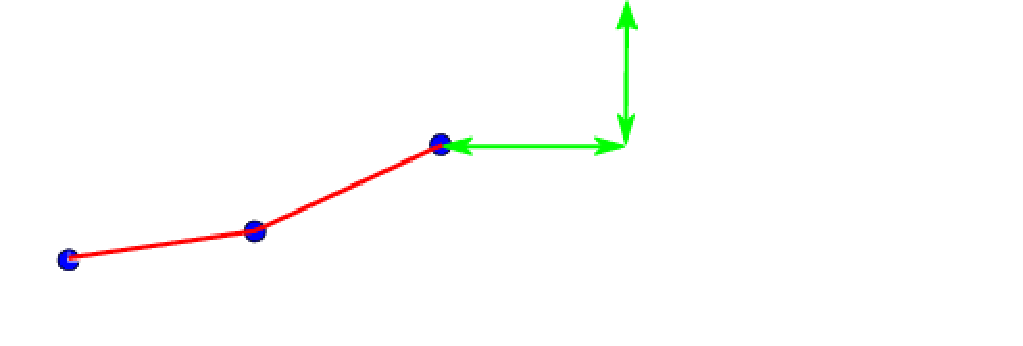
\includegraphics[width=0.9\linewidth]{fig/diskret_funksjon_1.pdf}}



\begin{itemize}
\item kan vi beregne neste verdi gjennom å regne ut $\Delta y_2$
\end{itemize}

\noindent
% !split

\paragraph{Visualisering av det numeriske skjemaet med $y_n$, $\Delta y_n$.}
% inline figure
\centerline{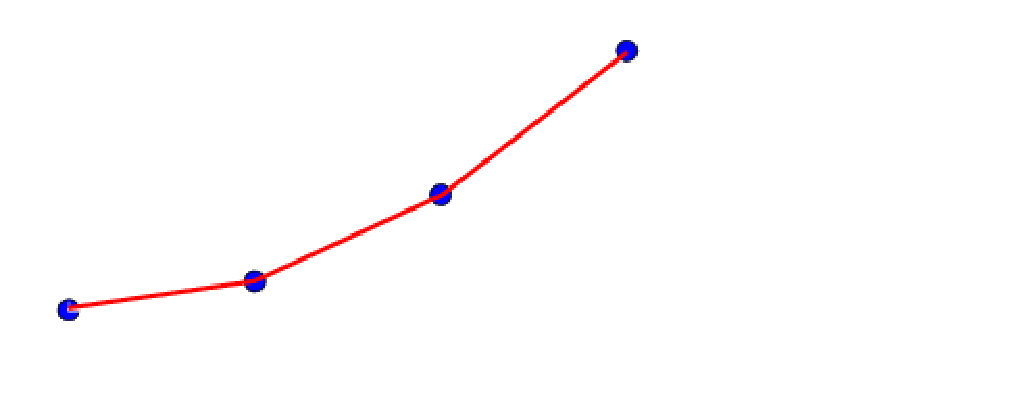
\includegraphics[width=0.9\linewidth]{fig/diskret_funksjon_3.pdf}}



\begin{itemize}
\item og legge til $y_2$. Vi har nå regnet ut $y_0 \ldots y_3$.
\end{itemize}

\noindent
% !split

\paragraph{Visualisering av det numeriske skjemaet med $y_n$, $\Delta y_n$.}
% inline figure
\centerline{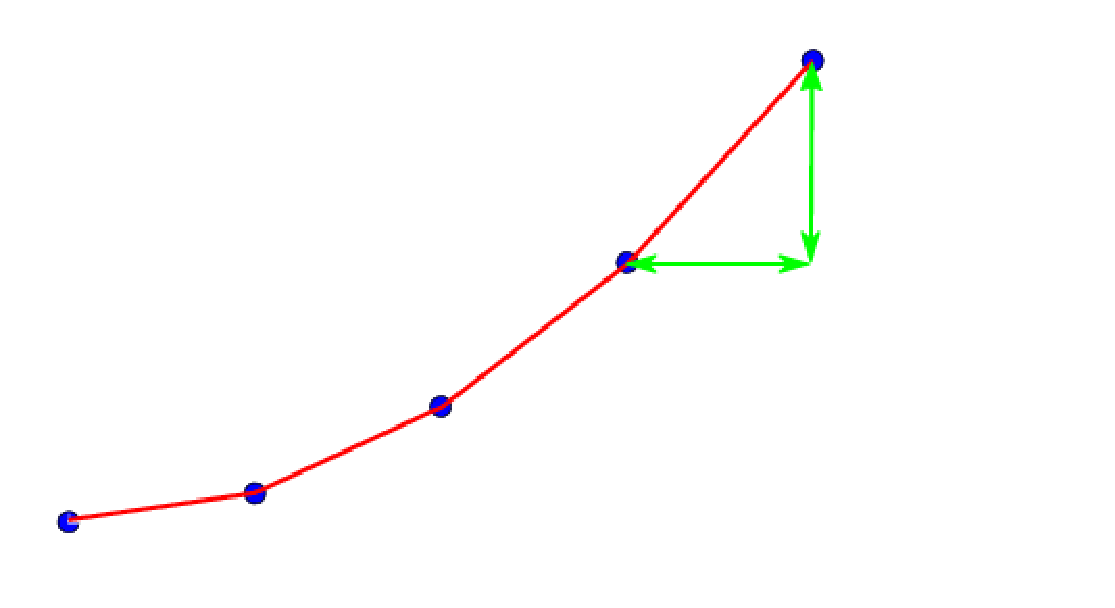
\includegraphics[width=0.9\linewidth]{fig/diskret_funksjon_5.pdf}}



\begin{itemize}
\item Og vi kan fortsette med neste verdi $y_4$. Og sånn går nå dagene...
\end{itemize}

\noindent
% !split

\paragraph{Er dette for vanskelig? Differensiallikninger tilhører pensum i R2 og kan være litt mye for elever i andre realfag?}
\begin{itemize}
\item Implementeringen av skjemaet krever også en del programmering.
\end{itemize}

\noindent
% !bpop
\begin{itemize}
\item Kan løsningen være et nytt MX-liknende fag, som kombinerer programmering med matematisk modellering?

\item To lektorer, Andreas Haraldsrud og Per Husum på Valler videregående skole i Sandvika mener dette!

\item De har forsøkt å få godkjent et eget 3h programfag i studiespesialiserende utdanningsprogram

\item De tenker at man kan ta dette faget samtidig som R2 og en av Fysikk 2, Biologi2, Kjemi2, eller Geofag 2.

\item ... men de har fått avslag for høst 2016.

\item Jeg håper at dette er en retning informatikkfaget kan gå mot og at det får gjennomslag for neste studieår og at Ludvigsen-utvalget får hørt om det når de skal se på de ulike fagplanene.

\item Hva tenker dere?
\end{itemize}

\noindent
% !epop

% !split

\section*{Prøve ut modellering av et strikkhopp hvor Python programmeringer brukes?}

Vi skal prøve å bruke Jupyter-notebook som skal kjøre Python skriptet i nettleseren deres. For å få til dette kan dere prøve 1 av 2 metoder:

% !bslidecell 00
\begin{itemize}
\item Metode 1 (mer omstendelig og mer pålitelig)
\begin{itemize}

 \item Last ned "index.ipynb" fra "'bit.ly/strikk_hopp'" : "'bit.ly/strikk_hopp'" og lagre den som "index.ipynb"

 \item Gå til \href{{https://try.jupyter.org}}{'https://try.jupyter.org'}

 \item Gå til Files og velg "open" og så last opp (upload)

 \item Last opp din fil "index.ipynb" og åpne den
\end{itemize}

\noindent
\end{itemize}

\noindent
% !eslidecell

% !bslidecell 01
\begin{itemize}
\item Metode 2 (mindre omstendelig men ganske treig å få satt igang)
\begin{itemize}

 \item Gå til \href{{http://mybinder.org}}{'http://mybinder.org'}

 \item Skriv inn "'johanhake/strikkhopp'" i "Tell us your GitHub repo"

 \item Trykk på "make my binder"

 \item Vent i 4 minutter...
\end{itemize}

\noindent
\end{itemize}

\noindent
% !eslidecell



% ------------------- end of main content ---------------

\end{document}

